\documentclass[11pt]{article}
\usepackage{amsmath}
\DeclareMathOperator*{\argmax}{argmax}
\DeclareMathOperator*{\argmin}{argmin} 
\usepackage{amsfonts}
\usepackage[utf8]{inputenc}
\usepackage[english]{babel}
\usepackage{amsthm}
\theoremstyle{definition}
\newtheorem{definition}{Definition}[section]
\usepackage{geometry}
\usepackage{mathtools}
\usepackage{listings}

\usepackage{xcolor}

\definecolor{codegreen}{rgb}{0,0.6,0}
\definecolor{codegray}{rgb}{0.5,0.5,0.5}
\definecolor{codepurple}{rgb}{0.58,0,0.82}
\definecolor{backcolour}{rgb}{0.95,0.95,0.92}

\lstdefinestyle{mystyle}{
    backgroundcolor=\color{backcolour},   
    commentstyle=\color{codegreen},
    keywordstyle=\color{magenta},
    numberstyle=\tiny\color{codegray},
    stringstyle=\color{codepurple},
    basicstyle=\ttfamily\footnotesize,
    breakatwhitespace=false,         
    breaklines=true,                 
    captionpos=b,                    
    keepspaces=true,                 
    numbers=left,                    
    numbersep=5pt,                  
    showspaces=false,                
    showstringspaces=false,
    showtabs=false,                  
    tabsize=2
}

\lstset{style=mystyle}

\usepackage{bbm}
\usepackage{physics}
\usepackage{parskip}
\usepackage{hyperref}
\usepackage[linesnumbered,ruled,vlined]{algorithm2e}
\DontPrintSemicolon
\usepackage{varioref}
\labelformat{algocf}{\textit{Algorithm}\,(#1)}

\usepackage{tikz}
\usetikzlibrary{shapes.geometric, arrows, calc, fit, positioning}
\tikzstyle{bluebox} = [rectangle, rounded corners, minimum width=3cm, minimum height=1cm,text centered, draw=black, fill=blue!30]
\tikzstyle{arrow} = [thick,->,>=stealth]

\author{Greg Strabel}
\title{Transformers}
\begin{document}
\maketitle

\section{Preliminaries}

\subsection{Matrix Multiplication}
Given two matrices $X \in \mathbb{R}^{n \times m}$ and $Y \in \mathbb{R}^{m \times k}$

\begin{equation}
\left( XY \right)_{ij} = \sum_{l=1}^m X_{il}Y_{lj} = X_{i \cdot} Y_{\cdot j}
\end{equation}

Therefore
\begin{equation}
\left( XY \right)_{\cdot j} = \sum_{l=1}^m Y_{lj} X_{\cdot l}
\end{equation}
so that the columns of $XY$ are linear combinations of the columns of $X$ and
\begin{equation}
\left( XY \right)_{i \cdot} = \sum_{l=1}^m X_{il} Y_{l \cdot}
\end{equation}
so that the rows of $XY$ are linear combinations of the rows of $Y$.

\subsection{Softmax}

\begin{definition}[Softmax] The $\mathrm{softmax}$ function $\sigma : \mathbb{R}^K \rightarrow \mathbb{R}^K$ is
\begin{equation}
\sigma(z)_i = \frac{e^{z_i}}{\sum_{j=1}^K e^{z_j}}
\end{equation}
\end{definition}

\subsection{Evaluating Text Quality}

\begin{definition}[n-grams] The n-grams of a string $y = y_1...y_K$ are
\begin{equation}
G_n(y) = \{ y_1...y_n, y_2...y_{n+1}, ... , y_{K-n+1}...y_K \}
\end{equation}
Note that $G_n(y)$ is a set, not a multiset, so the elements of $G_n(y)$ are distinct.
\end{definition}

\begin{definition}[Substring Count] Given two strings, $s = s_1...s_M$ and $y = y_1...y_K$ the substring count of substring $s$ in $y$ is
\begin{equation}
C(s,y) = | \{i \in \mathbb{N} \ | \ i > 0, \ i+M \leq K, \ y_i...y_{i+M} = s \} |
\end{equation}  
\end{definition}

\begin{definition}[Modified n-gram precision] Given a candidate corpus $\hat{S} = (\hat{y}^{(1)}, \hat{y}^{(2)}, ..., \hat{y}^{(M)})$ and corresponding reference corpi $S = (S_1, S_2, ..., S_M)$ where $S_i = (y^{(i,1)}, y^{(i,2)}, ..., y^{(i,N_i)})$, modified n-gram precision is defined as
\begin{equation}
p_n(\hat{S} , S) = \frac{\sum_{i=1}^M \sum_{s \in G_n(\hat{y}^{(i)})} \mathrm{min} (C(s, \hat{y}^{(i)}), \mathrm{max}_{y \in S_i} C(s,y))}{\sum_{i=1}^M \sum_{s \in G_n(\hat{y}^{(i)})} C(s, \hat{y}^{(i)})}
\end{equation}
\end{definition}

\begin{definition}[Brevity penalty] Given a candidate corpus $\hat{S} = (\hat{y}^{(1)}, \hat{y}^{(2)}, ..., \hat{y}^{(M)})$ and corresponding reference corpi $S = (S_1, S_2, ..., S_M)$ where $S_i = (y^{(i,1)}, y^{(i,2)}, ..., y^{(i,N_i)})$, the brevity penalty is defined as
\begin{equation}
BP(\hat{S}, S) = e^{-(r/c-1)^+}
\end{equation}
where
\begin{equation}
c = \sum_{i=1}^M | \hat{y}^{(i)} |
\end{equation}
is the length of the candidate corpus and
\begin{equation}
r = \sum_{i=1}^M | \mathrm{arg} \mathrm{min}_{y \in S_i} \left( | |y| - |\hat{y}^{(i)}| | \right) |
\end{equation}
is the effective reference corpus length.
\end{definition}

\begin{definition}[Bilingual Evaluation Understudy (BLEU)] Given a candidate corpus $\hat{S} = (\hat{y}^{(1)}, \hat{y}^{(2)}, ..., \hat{y}^{(M)})$, a corresponding reference corpi $S = (S_1, S_2, ..., S_M)$ where $S_i = (y^{(i,1)}, y^{(i,2)}, ..., y^{(i,N_i)})$, and $w \in \{ \left[ 0, 1\right]^{\infty} : \sum_{i=1}^{\infty} w_i = 1 \}$, the BLEU score is defined as:
\begin{equation}
BLEU_w (\hat{S}, S) = BP (\hat{S}, S) \cdot \mathrm{exp} \left( \sum_{n=1}^{\infty} w_n \mathrm{ln} p_n ( \hat{S} , S) \right)
\end{equation}
\end{definition}

\begin{definition}[ROUGE-n] Given a candidate sentence $\hat{y}$ and a corresponding corpus of reference sentences $S = \{ y^{(1)}, y^{(2)}, ..., y^{(N)} \}$, $ROUGE-n$ is defined as
\begin{equation}
ROUGE-n (\hat{y}, S) = \sum_{i=1}^N \frac{ \sum_{s \in G_n(y^{(i)})} \mathrm{min} (C(s,\hat{y}), C(s, y) )}{ \sum_{s \in G_n(y^{(i)})} C(s,y)}
\end{equation}
\end{definition}

Note that the definition of ROUGE metrics varies across sources. The definitions above align with \cite{schluter-2017-limits}.

\section{Attention}


\subsection{Dot-Product Attention}

\begin{definition}[Dot-Product Attention] Given $Q \in \mathbb{R}^{d_l \times d_k}$, $K \in \mathbb{R}^{d_s \times d_k}$ and $V \in \mathbb{R}^{d_s \times d_v}$

\begin{equation}
\mathrm{Attention} \left( Q,K,V \right) = \mathrm{softmax} \left( \frac{QK^T}{\sqrt{d_k}} \right) V \in \mathbb{R}^{d_l \times d_v}
\end{equation}
\end{definition}

\begin{figure}
\centering
  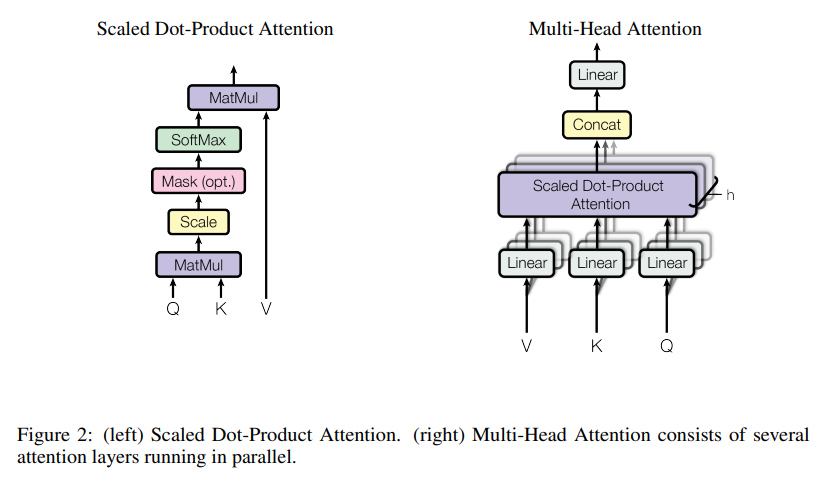
\includegraphics[width=\textwidth,height=\textheight,keepaspectratio]{transformers/attention_mechanism.png}
  \caption{Attention Mechanism \cite{vaswani2017attention}}
  \label{fig:attention}
\end{figure}

\subsection{Multihead Attention}
Given input matrices $X_Q \in \mathbb{R}^{d_l \times d_g}$, $X_K \in \mathbb{R}^{d_s \times d_w}$ and $X_V \in \mathbb{R}^{d_s \times d_u}$ and weight matrices
\begin{gather}
\nonumber \{W_Q^i \in \mathbb{R}^{d_g \times d_k} \}_{i=1}^h \\
\{W_K^i \in \mathbb{R}^{d_w \times d_k} \}_{i=1}^h \\
\nonumber \{W_V^i \in \mathbb{R}^{d_u \times d_v} \}_{i=1}^h \\
W_O \in \mathbb{R}^{hd_v \times d_o}
\end{gather}
we define
\begin{gather}
\nonumber Q^i = X_QW_Q^i \in \mathbb{R}^{d_l \times d_k} \\
K^i = X_KW_K^i \in \mathbb{R}^{d_s \times d_k} \\
\nonumber V^i = X_VW_V^i \in \mathbb{R}^{d_s \times d_v}
\end{gather}

\begin{equation}
A^i = \mathrm{Attention} \left(Q^i,K^i,V^i \right) \in \mathbb{R}^{d_l \times d_v}
\end{equation}

\begin{equation}
\mathrm{Multihead}\left(X_Q, X_K, X_V \right) =
\mathrm{concat} \left( A_1, ... , A_h \right)W_O
\in \mathbb{R}^{d_l \times d_o}
\end{equation}

\subsection{Multihead Self-Attention}

In Multihead Self-Attention, $X_Q = X_K = X_V$ so that $d_{model} \coloneqq d_g = d_w = d_u$, $L \coloneqq d_l = d_s$ and $\mathrm{Multihead}\left(X_Q, X_K, X_V \right) \in \mathbb{R}^{L \times d_o}$. If we also have $d_o = d_{model}$ then we get the Multihead Self-Attention described in \cite{vaswani2017attention}{Attention Is All You Need}

\subsection{Transformer Block}

A single transformer block (see Figure \ref{fig:transformerblock}) takes an input tensor $X_0$ and then:
\begin{enumerate}
\item Applies a multi-head attention layer to $X_0$ to produce $X_1$
\item Adds $X_0$ and $X_1$ and applies normalization to produce $X_2$
\item Applies a fully connected feed forward layer to $X_2$ to produce $X_3$
\item Adds $X_2$ and $X_3$ and applies normalization to produce the final output $X_4$
\end{enumerate}

\begin{figure}
\centering
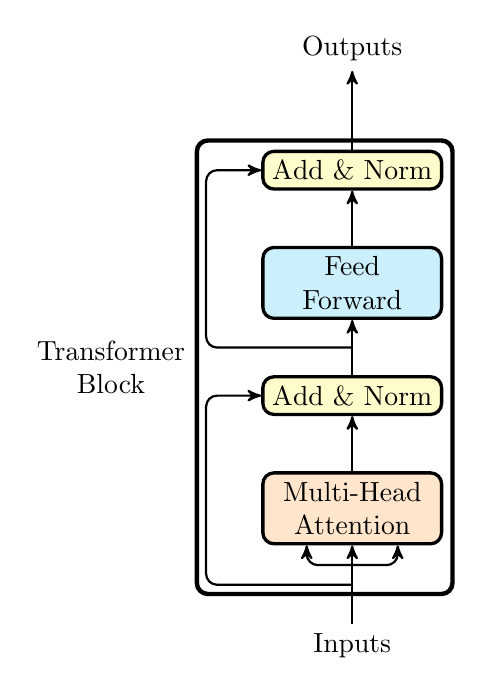
\begin{tikzpicture}[
 module/.style={draw, very thick, rounded corners, minimum width=15ex},
 embmodule/.style={module, fill=red!20},
 mhamodule/.style={module, fill=orange!20},
 lnmodule/.style={module, fill=yellow!20},
 ffnmodule/.style={module, fill=cyan!20},
 arrow/.style={-stealth', thick, rounded corners},
 ]
 \node (inputs) {Inputs};
 %\node[above= 2.0cm of inputs, embmodule, align=center]
 %(inputemb) {Input\\Embedding};
 %\node[above of=inputs, draw, thick, circle] (embplus)
 %{$+$};
 %\node[above of=embplus, mhamodule, align=center] (mha)
 %{Multi-Head\\Attention};
 \node[above= 1.0cm of inputs, mhamodule, align=center] (mha)
 {Multi-Head\\Attention};
 \node[above= 0.7cm of mha, lnmodule, align=center] (addnorm1)
 {Add \& Norm};
 \node[above= 0.7cm of addnorm1, ffnmodule, align=center] (ffn)
 {Feed\\Forward};
 \node[above= 0.7cm of ffn, lnmodule, align=center] (addnorm2)
 {Add \& Norm};
 \node[above= 1.0cm of addnorm2] (outputs) {Outputs};
 %\node[left of= embplus, draw, thick, circle, inner sep=0pt,label={[align=left]left:Positional\\Encoding}]
  %(pe) {\tikz \draw[scale=0.1] plot[domain=0.0:10.0]
  %(\x,{sin(\x r)});};
  \draw[arrow] (inputs) -- (mha);
  %\draw[arrow] (inputs) -- (inputemb);
 %\draw[arrow] (inputemb) -- (embplus);
 %\draw[arrow] (pe) -- (embplus);
 %\draw[arrow] (embplus) -- (mha);
 \draw[arrow] (mha) -- (addnorm1);
 \draw[arrow] (addnorm1) -- (ffn);
 \draw[arrow] (ffn) -- (addnorm2);
 \draw[arrow] (addnorm2) -- (outputs);

%\coordinate (mharesidual) at
% ($(mha.south)!0.5!(embplus.north)$);
\coordinate (mharesidual) at
 ($(mha.south)!0.5!(inputs.north)$);
\coordinate (ffnresidual) at
($(ffn.south)!0.5!(addnorm1.north)$);
\coordinate (mhafork) at
($(mha.south)!0.5!(mharesidual)$);
\coordinate[left = 0.7cm of addnorm1] (ln1residualleft);
\coordinate[left = 0.7cm of addnorm2] (ln2residualleft);

\node[fit=(mha)(addnorm2)(mharesidual)(ln1residualleft), draw, ultra thick, rounded corners,
label={[align=center]left:Transformer\\Block}] (encoder) {};

\draw[arrow]
 (mharesidual)-|(ln1residualleft)--(addnorm1);
 \draw[arrow]
 (ffnresidual)-|(ln2residualleft)--(addnorm2);
 \draw[arrow] (mhafork)-|($(mha.south)!0.5!(mha.south
 west)$);
 \draw[arrow] (mhafork)-|($(mha.south)!0.5!(mha.south
 east)$);

\end{tikzpicture}
\caption{Single Transformer Block}
\label{fig:transformerblock}
\end{figure}



\section{Attention is All You Need \cite{vaswani2017attention}}

Multi-head self-attention was introduced in the paper Attention is All You Need \cite{vaswani2017attention}, which used the architecture in Figure \ref{fig:fulltransformer} for a translation task.

\begin{figure}
\centering
  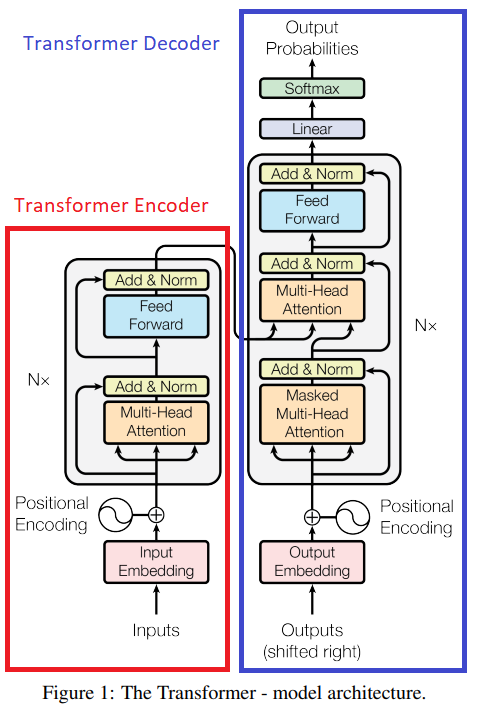
\includegraphics{transformers/transformer_architecture.png}
  \caption{Transformer Architecture \cite{vaswani2017attention}}
  \label{fig:fulltransformer}
\end{figure}

Inputs to the model are Byte Pair Encoded (BPE, section \ref{BPE}) tokens, which are mapped to a learned embedding space. In order for the model to make use of the order of the input sequence, information on sequence order is injected by adding in sine and cosine function of different frequencies:

\begin{equation}
\begin{array}{l}
PE_{(pos,2i)} = \mathrm{sin}(pos/10000^{2i/d_{model}}) \\ \\ 
PE_{(pos,2i+1)} = \mathrm{cos}(pos/10000^{2i/d_{model}})
\end{array}
\end{equation}

\section{Improving Language Understanding by Generative Pre-Training}

\cite{radford2018gpt} is the OpenAI article that introduced GPT (Generative Pre-Training). This framework uses unsupervised pre-training of a multi-layer transformer decoder with a masked language model objective followed by fine-tuning for specific tasks.

\textbf{Unsupervised pre-training} involves taking a corpus of tokens $\mathcal{U} = \{u_1, u_2, ..., u_n \}$ and training a model to maximize the likelihood objective:
\begin{equation}
L_1(\mathcal{U}) = \sum_i \mathrm{log} P (u_i|u_{i-k}, ...,u_{i-1}; \Theta)
\end{equation}
where $k$ is the size of the context window, $P$ is the conditional probability of the next token and $\Theta$ are the parameters of the model.

\cite{radford2018gpt} use a multi-layer transformer decoder for their model; a stack of multiple transformer blocks:

\begin{equation}
\begin{array}{l}
h_0 = UW_e + W_p \\
h_l = \mathtt{transformer\_decoder}(h_{l-1}) \ \ \forall i \in \left[1,...,n \right] \\
P(u) = \mathtt{softmax}(h_nW_e')
\end{array}
\end{equation}
where $U = (u_{-k},...,u_{-1})$ is the context vector of tokens, $n$ is the number of layers, $W_e$ is the token embedding matrix, and $W_p$ is the position embedding matrix.

\textbf{Supervised fine-tuning} uses labeled training data to further optimize the model for certain tasks, including classification, semantic similarity, textual entailment and question answering. Given a labeled dataset $\mathcal{C}$ of inputs $\{x^1, ...,x^m \}$ and targets $y$, the model is trained to maximize the likelihood objective:
\begin{equation}
L_2(\mathcal{C}) = \sum_{(x,y)} \mathrm{log} P (y|x^1,...,x^m)
\end{equation}
where
\begin{equation}
P (y|x^1,...,x^m) = \mathrm{softmax}(h_l^mW_y)
\end{equation}
$h_l^m$ is the last output of the final transformer block and $W_y$ are learned parameters. 

During fine-tuning, the authors continued to use the masked language modeling to improve generalization and accelerate convergence. Hence, the final fine-tuning objective was 
\begin{equation}
L_3(\mathcal{C}) = L_2{\mathcal{C}} + \lambda L_1(\mathcal{C})
\end{equation}
with a tuning parameter $\lambda$ that trades off between the two objectives of performance on the fine-tuning task and generalization.

\begin{figure}
\centering
  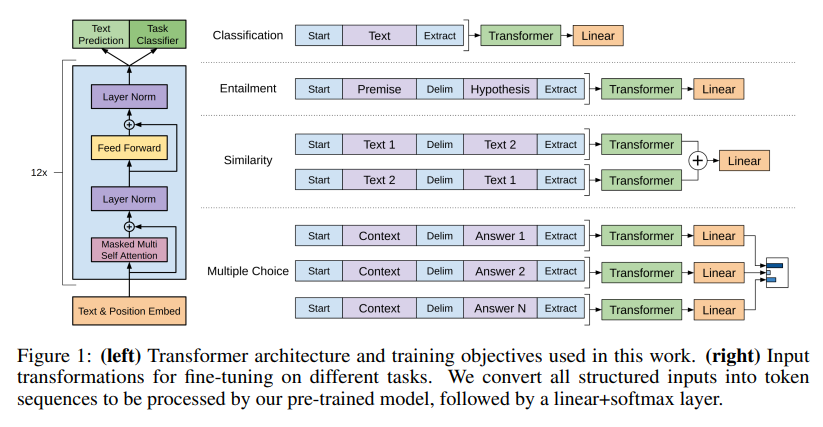
\includegraphics[width=\textwidth,height=\textheight,keepaspectratio]{transformers/gpt_objectives.png}
  \caption{GPT Training Objectives \cite{radford2018gpt}}
  \label{fig:gptobjectives}
\end{figure}

\section{Language Models are Unsupervised Multitask Learners \cite{radford2019gpt2}}

\cite{radford2019gpt2} is the paper from OpenAI that introduced GPT-2. The principle finding of this paper was that by scaling up both model size from approximately 100M parameters to 1.5B parameters and using a significantly larger pre-training dataset (WebText - based on Common Crawl data with outbound Redit links), a Transformer-decoder type model could achieve state-of-the-art performance on many tasks without the need to fine-tune.

\section{Language models are few-shot learners \cite{brown2020gpt3}}

\cite{brown2020gpt3} is the paper from OpenAI that introduced GPT-3. GPT-3 is again a transformer decoder-only model pre-trained on a curated version of the Common Crawl dataset. Again, OpenAI significantly scaled up the size of the model - the largest GPT-3 model has 175B parameters. Like GPT-2, GPT-3 was not fine-tuned for any specific task, but still demonstrated near-SOTA performance across a range of NLP tasks. GPT-3 performed better with infew-shot contexts; that is, when examples demonstrating desired output for the task was provided as part of the prompt.

\section{Training language models to follow instructions with human feedback \cite{ouyang2022training}}

This is the paper from OpenAI that introduced Instruct GPT and the use of Reinforcement Learning from Human Feedback (RLHF). Instruct GPT uses a pre-trained GPT 3 model and fine-tunes it in three steps:
\begin{enumerate}
\item Given a set of prompts and desired responses, the model is fine-tuned on these examples in a supervised manor (SFT).
\item Given a prompt, several model outputs are sampled and a human labeler ranks them from best to worst. A dataset generated in this manor is then used to train a reward model (RM) (also a GPT 3 model).
\item Given a prompt, the model from 1 generates an output, the reward model calculates a reward and then the model is updated using reinforcement learning via proximal policy optimization.
\end{enumerate}

\begin{figure}
\centering
  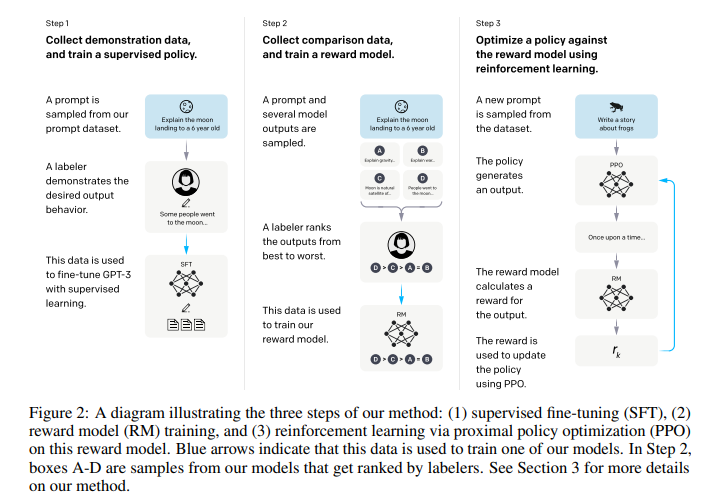
\includegraphics[width=\textwidth,height=\textheight,keepaspectratio]{transformers/instructgpt.png}
  \caption{Instruct GPT Fine-Tuning \cite{ouyang2022training}}
  \label{fig:instructgpt}
\end{figure}

\section{BERT: Pre-training of Deep Bidirectional Transformers for Language Understanding}

\cite{devlin2019bert} was the first paper to introduce BERT models - transformer encoder only models that can be fine-tuned for a variety of tasks.

\section{Scaling Transformers to Longer Sequences}

One limitation of the original transformers is that their computational complexity grows quadratically in the length of the input sequence; that is, they have computational complexity of $O(n^2)$, where $n$ is the sequence length. There have been several approaches developed to reduce this complexity.

\subsection{Transformer-XL \cite{dai2019transformerxl}}

One crude option to reduce computational complexity during training is to split text into segments of length $L$ and train a model on the individual segments, ignoring all contextual information from previous segments. This reduces complexity during training but causes contextual fragmentation as no information flows across segments. This vanilla model is shown in \ref{fig:transformerxl-vanilla}. At each time step during evaluation, the model processes a text segment of length $L$, the last output position is recorded and then the context window is shifted to the right by one step and the process repeated. By shifting only a single time step, each prediction is able to use the context of the last $L$ positions, alleviating the contextual fragmentation in training, but reintroducing computational complexity. 

\begin{figure}
\centering
  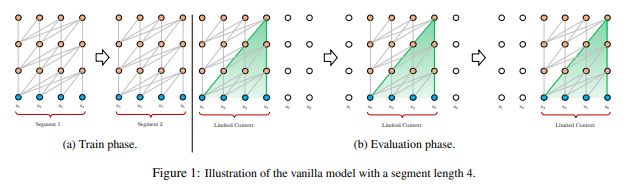
\includegraphics[width=\textwidth,height=\textheight,keepaspectratio]{transformers/transformerXL_vanilla.png}
  \caption{Transformer with Fixed Context Window \cite{dai2019transformerxl}}
  \label{fig:transformerxl-vanilla}
\end{figure}

In order to address the issue of contextual fragmentation, \cite{dai2019transformerxl} introduce a recurrence mechanism. With two consecutive segments of length $L$, $s_{\tau} = \left[ x_{\tau,1},...,x_{\tau,L} \right]$ and $s_{\tau+1} = \left[x_{\tau+1,1},...,x_{\tau+1,L}\right]$, let the $n$-th layer hidden state sequence produced by the $\tau$-th segment $s_{\tau}$ be $h_{\tau}^n \in \mathbb{R}^{L \times d}$, where $d$ is the hidden dimension. Then

\begin{equation}
\begin{array}{l}
\tilde{h}_{\tau+1}^{n-1} = \left[ SG(h_{\tau}^{n-1}) \circ h_{\tau+1}^{n-1} \right] \\
\\

q_{\tau+1}^n,k_{\tau+1}^n,v_{\tau+1}^n = h_{\tau+1}^{n-1}W_q', \tilde{h}_{\tau+1}^{n-1}W_k', \tilde{h}_{\tau+1}^{n-1}W_v' \\
\\
h_{\tau+1}^n = \mathtt{transformer\_block}(q_{\tau+1}^n,k_{\tau+1}^n,v_{\tau+1}^n)
\end{array}
\end{equation}

where $SG$ is the stop-gradient function and $\circ$ denotes concatenation of vectors. Compared to the vanilla transformer, the keys and values in TransformerXL are constructed with an extended context, creating what is essentially a segment-level recurrence in hidden states.

\begin{figure}
\centering
  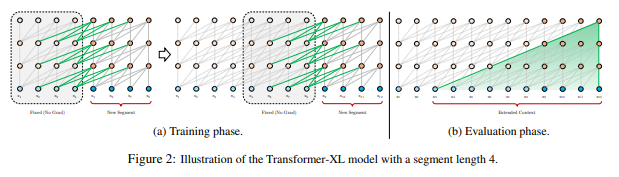
\includegraphics[width=\textwidth,height=\textheight,keepaspectratio]{transformers/transformerXL_model.png}
  \caption{TransformerXL \cite{dai2019transformerxl}}
  \label{fig:transformerxl}
\end{figure}


\subsection{Generating Long Sequences with Sparse Transformers}

In \cite{child2019generating}, the authors scale transformers to longer sequences by factorizing the self-attention mechanism. Let $S = \{S_1,...,S_L \}$, where $S_i \subseteq \{1,...,L \} \ \forall i \leq L$. Then

\begin{equation}
\mathrm{Attend}(X,S) = \left( a(X_{\cdot i}, S_i) \right)_{i \in \{1,...,L\}}
\end{equation}

\begin{equation}
a(X_{\cdot i}, S_i) = \mathrm{softmax}\left( \frac{(W_qX_{\cdot i})K_{S_i}'}{\sqrt{d}} \right) V_{S_i}
\end{equation}

\begin{equation}
K_{S_i} = \left( W_k X_{\cdot j} \right)_{j \in S_i} \ \ \ \ V_{S_i} = \left( W_v X_{\cdot j} \right)_{j \in S_i}
\end{equation}

For full self-attention in an autoregressive model, $S_i = \{ j : j \leq i \}$ so that each element attends to all previous positions and its own position.

On the other hand, factorized self-attention uses $p$ separate attention heads, where the $m$th head defines a subset of the indices $A_i^{(m)} \subset \{j : j \leq i \}$. In particular, the authors consider two factorizations:

\begin{itemize}
\item Strided Attention sets $A_i^{(1)} = \{t,t+1,...,i \}$ for $t = \mathrm{max}(0,i-l)$ and $A_i^{(2)} = \{j : (i-j) \mathrm{mod} l =0 \}$.
\item Fixed Attention sets $A_i^{(1)} = \{j : (\lfloor j/l \rfloor = \lfloor i/l \rfloor) \}$ and $A_i^{(2)} = \{ j : j \mathrm{mod} l \in \{ t, t+1,...,l \}, t = l-c \}$.
\end{itemize}

where $l$ is the stride length and c is a hyperparameter. Strided attention performs best for data with structure that aligns with the stride, like images. Fixed attention performs well on data without a periodic structure, such as text.

\begin{figure}
\centering
  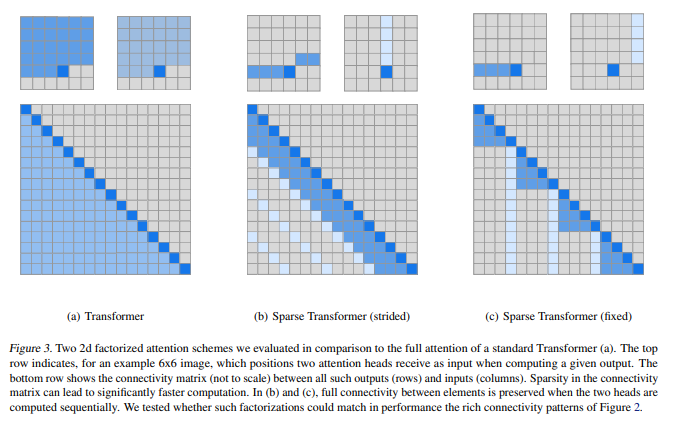
\includegraphics[width=\textwidth,height=\textheight,keepaspectratio]{transformers/sparse_transformer_attention.png}
  \caption{Sparse Transformer Attention \cite{child2019generating}}
  \label{fig:sparse_transformer_attention}
\end{figure}

\subsection{Longformer \cite{beltagy2020longformer}}

Longformer is a paper from AllenAI that introduced the Longformer model. Similar to sparse transformers, Longformer alters the attention pattern so that not all positions attend to all other positions. Longformer reduces the computational complexity $O(n^2)$ of full attention to $O(n \times w)$ by using a sliding window of size $w$. The paper also dilates the windows with gaps of size dilation $d$ so that the final receptive field is $l \times d \times w$.

\begin{figure}
\centering
  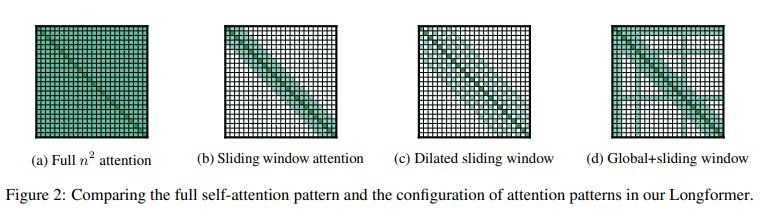
\includegraphics[width=\textwidth,height=\textheight,keepaspectratio]{transformers/longformer.png}
  \caption{Longformer Attention \cite{beltagy2020longformer}}
  \label{fig:longformer}
\end{figure}

\subsection{Big Bird: Transformers for Longer Sequences}

\begin{figure}
\centering
  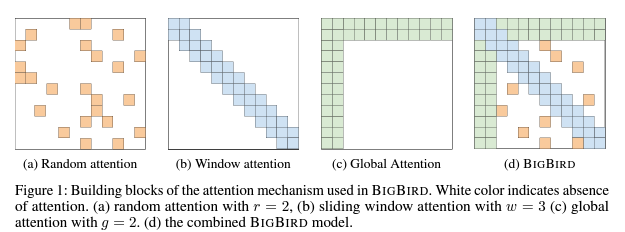
\includegraphics[width=\textwidth,height=\textheight,keepaspectratio]{transformers/big_bird.png}
  \caption{Big Bird Attention \cite{bigbird}}
  \label{fig:bigbird}
\end{figure}

\section{Distilling}

\subsection{Distilling Step-by-Step! Outperforming Larger Language Models with Less Training Data and Smaller Model Sizes}

\begin{figure}
\centering
  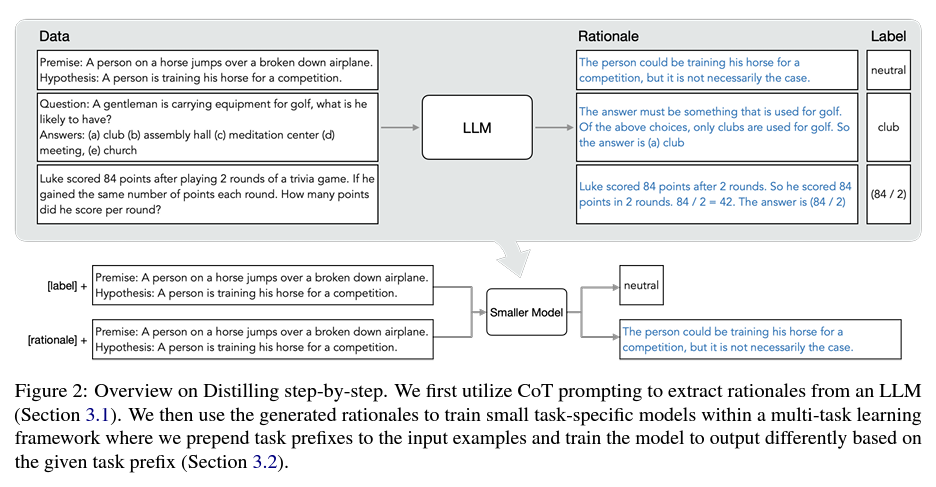
\includegraphics[width=\textwidth,height=\textheight,keepaspectratio]{transformers/distilling_step_by_step.png}
  \caption{Distilling Step-by-Step \cite{hsieh2023distilling}}
  \label{fig:distilling_step_by_step}
\end{figure}

\section{Improving Fine-tuning}

\subsection{LoRA: Low-Rank Adaptation of Large Language Models \cite{hu2021lora}}

LoRA is a method for fine-tuning large, pre-trained transformers with limited fine-tuning data and/or compute. LoRA freezes pre-trained model weights and injects trainable rank decomposition matrices into each layer of the transformer architecture, significantly reducing the number of trainable parameters for downstream tasks.

Given a pre-trained weight matrix $W_0 \in \mathbb{R}^{d \times k}$, during fine-tuning we replace $W_0$ with $\mathrm{frozen}(W_0) + BA$ where $B \in \mathbb{R}^{d \times r}$ and $A \in \mathbb{R}^{r \times k}$ are trainable parameters, $\mathrm{rank}(r) \ll \mathrm{min}(d,k)$, $A$ has a random Gaussian initialization and $B$ is initialized to zero.

\begin{figure}
\centering
  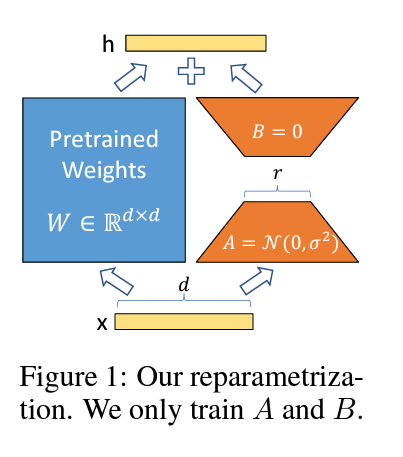
\includegraphics[width=0.4\textwidth]{transformers/lora_overview.png}
  \caption{LoRA Fine-tuning Strategy \cite{DBLP:journals/corr/abs-2106-09685}}
  \label{fig:lora-overview}
\end{figure}

\subsection{QLoRA}

\begin{figure}
\centering
  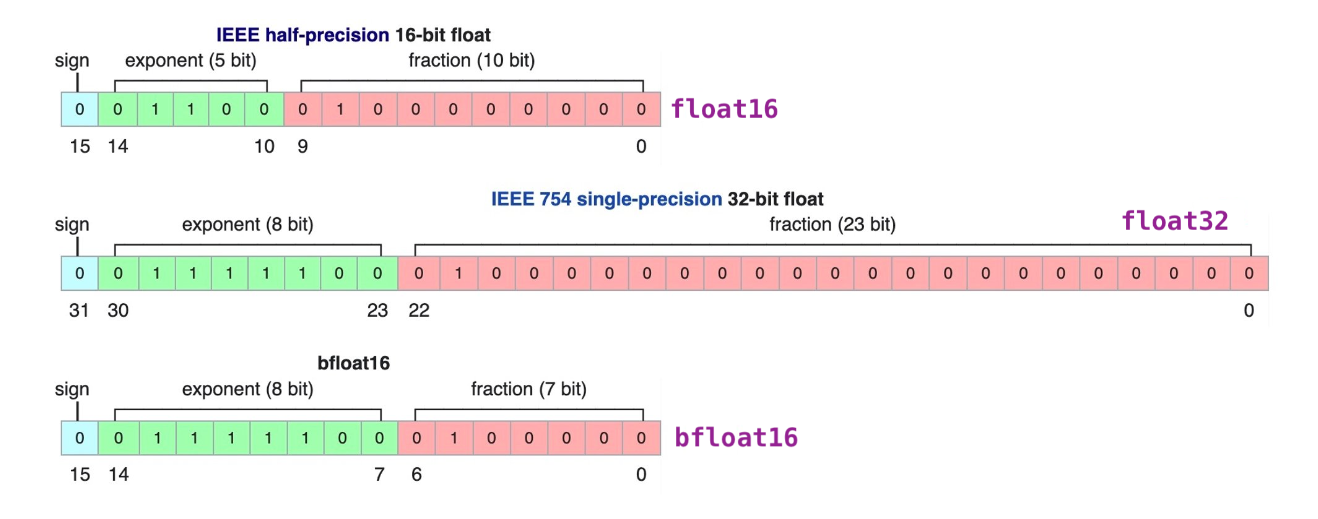
\includegraphics[width=\textwidth,height=\textheight,keepaspectratio]{transformers/bfloat16.png}
  \caption{bfloat16 \cite{bfloat16img}}
  \label{fig:bfloat16}
\end{figure}

\section{Relative Position Embeddings}

Relative position embeddings were introduced by \cite{shaw2018selfattention}.

Given relative position embedding matrix $E^r \in \mathbb{R}^{L \times d_{model}}$ and matrix $X \in \mathbb{R}^{L \times d_{model}}$

\begin{algorithm}
\SetNoFillComment
\KwIn{Relative embedding matrix $E^r \in \mathbb{R}^{L \times d_{model}}$ \\
\mbox{}\phantom{\textbf{Input:}} Matrix $X \in \mathbb{R}^{L \times d_{model}}$} 
\KwOut{$D \in \mathbb{R}^{L \times L}$}
$A \leftarrow XE^{rT} \in \mathbb{R}^{L \times L}$\;
$M \leftarrow \begin{cases} m_{i,j} = 1 & i \leq L, j \leq L, i \geq j \\ m_{i,j} = 0 & i \leq L, j \leq L, i < j \end{cases} \in \mathbb{R}^{L \times L}$\;
$A \leftarrow A \odot M$ \ \ \ // element-wise product\;
$B \leftarrow \begin{cases} b_{i,j} = 0 & j=1, i \leq L \\ b_{i,j} = a_{i,j-1} & i \leq L, 1 < j \leq L+1 \end{cases} \in \mathbb{R}^{L \times L+1}$\;
$V \leftarrow \mathrm{vec} (B^T)$\;
$C \leftarrow \{c_{ij} = V_{(i-1)L + j} \ | \ i \leq L, j \leq L \} \in \mathbb{R}^{L+1 \times L}$\;
$D \leftarrow \{d_{ij} = c_{i+1,j} \ | \ i \leq L, j \leq L\}$\;
\Return{$D$}\;
\caption{Relative Position Embedding of \cite{huang2018music}}\label{rel-pos-emb}
\end{algorithm}

\begin{figure}
\centering
  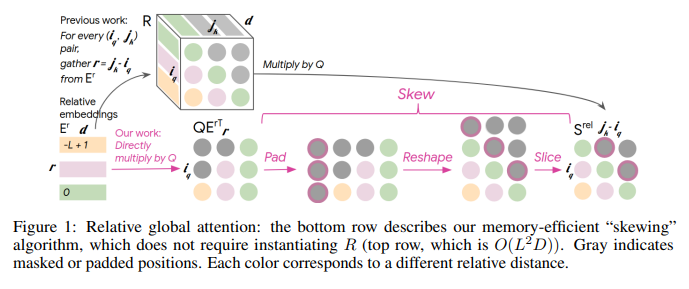
\includegraphics[width=\textwidth,height=\textheight,keepaspectratio]{transformers/relative_global_attention.png}
  \caption{Relative Global Attention \cite{huang2018music}}
  \label{fig:relative_global_attention}
\end{figure}

\section{Prompt Design and Tuning}

Need to cover \cite{li2021prefixtuning} and \cite{lester2021power}


\section{Byte-Pair Encoding} \label{BPE}

\begin{minipage}{\linewidth}
\begin{lstlisting}[language=Python, caption=Byte-Pair Encoding]
import re, collections

def get_stats(vocab):
    pairs = collections.defaultdict(int)
    for word, freq in vocab.items():
        symbols = word.split()
        for i in range(len(symbols)-1):
            pairs[symbols[i],symbols[i+1]] += freq
    return pairs

def merge_vocab(pair, v_in):
    v_out = {}
    bigram = re.escape(' '.join(pair))
    p = re.compile(r'(?<!\S)' + bigram + r'(?!\S)')
    for word in v_in:
        w_out = p.sub(''.join(pair), word)
        v_out[w_out] = v_in[word]
    return v_out

vocab = {'l o w </w>' : 5, 'l o w e r </w>' : 2,
         'n e w e s t </w>':6, 'w i d e s t </w>':3}

num_merges = 10

for i in range(num_merges):
    pairs = get_stats(vocab)
    best = max(pairs, key=pairs.get)
    vocab = merge_vocab(best, vocab)
    print(best)

\end{lstlisting}
\end{minipage}

\section{Numeric Types and Precision}

\begin{figure}
\centering
  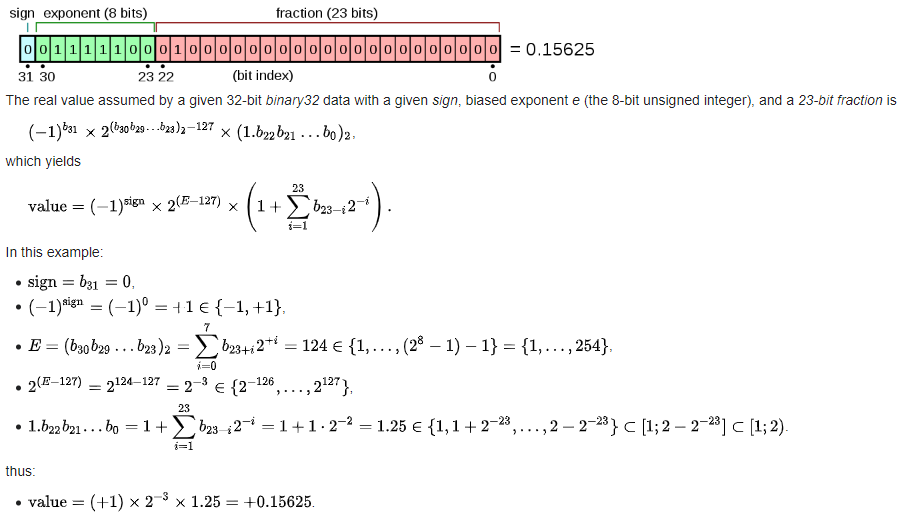
\includegraphics[width=\textwidth,height=\textheight,keepaspectratio]{transformers/fp32-wikipedia.png}
  \caption{float32 \cite{float32img}}
  \label{fig:float32}
\end{figure}


More papers to cover:

\begin{enumerate}
\item Roformer
\item FLAN T5 - Fine-tuning Language Net - instruction tuning
\item Roberta
\item Albert
\item Switch Transformer
\item GLaM
\item QLoRA
\item Unigrams
\item SentencePiece
\end{enumerate}


\bibliographystyle{alpha} % We choose the "plain" reference style
\bibliography{transformers} % Entries are in the refs.bib file


\end{document}